\section{Sprint 6 : Surveillance et maintenance prédictive}

\subsection{Introduction}

Après la mise en place des fonctions de maintenance préventive, corrective et de pilotage, ce sixième Sprint est consacré à la surveillance des équipements et à la maintenance prédictive.

La plateforme collecte des données techniques émises par des capteurs et des équipements connectés. Ces données sont diffusées en temps réel aux utilisateurs autorisés afin de suivre l'état des machines et de détecter des situations nécessitant une vérification. Un service indépendant, développé avec FastAPI, assure l'analyse d'anomalies sur des données de roulements.

Ce Sprint vise ainsi à compléter la maintenance préventive par une approche fondée sur l'état observé des équipements. Les résultats produits par les modèles constituent une aide au diagnostic et restent soumis à la validation des administrateurs et des techniciens.

Le chapitre présente les objectifs et le Sprint Backlog, puis la conception de la chaîne de collecte et d'analyse. Il décrit ensuite les fonctionnalités réalisées, les mécanismes de validation humaine ainsi que les limites actuelles du modèle d'anomalies.

\subsection{Objectifs du Sprint}

L'objectif principal de ce Sprint est de mettre en place une surveillance en temps réel des équipements et d'intégrer une première capacité d'analyse prédictive.

Les objectifs spécifiques sont les suivants :

\begin{itemize}
    \item gérer les capteurs et les équipements connectés ;
    \item recevoir les mesures et les événements transmis par les équipements ;
    \item conserver les mesures avec leur horodatage et leur statut ;
    \item diffuser les changements d'état en temps réel ;
    \item superviser l'état des machines sur une interface dédiée ;
    \item calculer un indicateur de santé pour chaque machine ;
    \item intégrer un service d'analyse d'anomalies basé sur l'apprentissage automatique ;
    \item enregistrer les scores, les niveaux de risque et les raisons détectées ;
    \item générer une alerte lorsqu'une anomalie persiste ;
    \item permettre la confirmation ou le rejet d'une analyse par un utilisateur habilité ;
    \item conserver l'historique des analyses associées à chaque machine.
\end{itemize}

À la fin du Sprint, l'administrateur et le technicien doivent pouvoir consulter l'état des équipements supervisés, lancer une analyse et décider du suivi à donner à une anomalie détectée.

\subsection{Sprint Backlog}

Le tableau~\ref{tab:sprint6-backlog} recense les tâches planifiées pour ce Sprint.

{\footnotesize
\setlength{\tabcolsep}{4pt}
\begin{longtable}{|p{0.9cm}|>{\raggedright\arraybackslash}p{9.1cm}|>{\raggedright\arraybackslash}p{1.6cm}|>{\raggedright\arraybackslash}p{1.6cm}|}
\caption{Sprint Backlog du Sprint 6}
\label{tab:sprint6-backlog}\\
\hline
\textbf{ID} & \textbf{Tâche} & \textbf{Priorité} & \textbf{Statut} \\
\hline
\endfirsthead

\hline
\textbf{ID} & \textbf{Tâche} & \textbf{Priorité} & \textbf{Statut} \\
\hline
\endhead

S6-01 &
Gérer les capteurs, leurs types et leur activation. &
Haute & Réalisé \\
\hline

S6-02 &
Gérer les équipements connectés et leurs clés d'authentification. &
Haute & Réalisé \\
\hline

S6-03 &
Mettre en place l'ingestion des mesures par MQTT. &
Haute & Réalisé \\
\hline

S6-04 &
Diffuser les événements en temps réel par WebSocket. &
Haute & Réalisé \\
\hline

S6-05 &
Développer la supervision en direct de l'état des machines. &
Haute & Réalisé \\
\hline

S6-06 &
Mettre en place le calcul de l'indicateur de santé des machines. &
Moyenne & Réalisé \\
\hline

S6-07 &
Développer le service FastAPI d'analyse des anomalies. &
Haute & Réalisé \\
\hline

S6-08 &
Intégrer l'appel authentifié entre le backend et le service d'analyse. &
Haute & Réalisé \\
\hline

S6-09 &
Enregistrer les analyses, les scores et les niveaux de risque. &
Haute & Réalisé \\
\hline

S6-10 &
Mettre en place la validation humaine des analyses. &
Haute & Réalisé \\
\hline

S6-11 &
Générer des notifications pour les anomalies persistantes. &
Moyenne & Réalisé \\
\hline

S6-12 &
Intégrer l'assistant Gemini de manière optionnelle. &
Faible & Réalisé \\
\hline

S6-13 &
Vérifier la collecte, l'inférence et la validation par des tests. &
Haute & Réalisé \\
\hline

\end{longtable}}

User Stories associées :

\begin{itemize}
    \item \textbf{US23 :} en tant qu'administrateur, je souhaite gérer les capteurs et les équipements connectés afin d'organiser la collecte des données ;
    \item \textbf{US24 :} en tant que technicien, je souhaite suivre l'état des machines en temps réel afin de réagir rapidement à un changement anormal ;
    \item \textbf{US25 :} en tant que technicien, je souhaite consulter l'indicateur de santé d'une machine afin d'orienter mes contrôles ;
    \item \textbf{US26 :} en tant qu'administrateur ou technicien, je souhaite lancer une analyse d'anomalies et consulter ses résultats afin d'appuyer mon diagnostic ;
    \item \textbf{US27 :} en tant qu'administrateur ou technicien, je souhaite confirmer ou rejeter une analyse afin de conserver une décision humaine traçable.
\end{itemize}

\subsection{Conception du Sprint}

\subsubsection{Diagramme des cas d'utilisation}

La figure~\ref{fig:usecase-monitoring} présente les cas d'utilisation du domaine de la surveillance et de la maintenance prédictive. L'administrateur gère les capteurs et les équipements connectés, supervise les machines, consulte l'indicateur de santé, lance une analyse, consulte l'historique, valide ou rejette un résultat et sollicite l'assistant intelligent. Le technicien suit l'état des machines en temps réel, consulte la santé de ses équipements, lance une analyse, consulte l'historique et décide du sort d'une analyse. Un équipement connecté ou un capteur alimente la plateforme par ses mesures et ses événements, tandis que le service d'analyse des anomalies intervient comme acteur externe lors du lancement d'une analyse.
\begin{figure}[H]
    \centering
    \IfFileExists{figures/usecase-monitoring.png}{%
        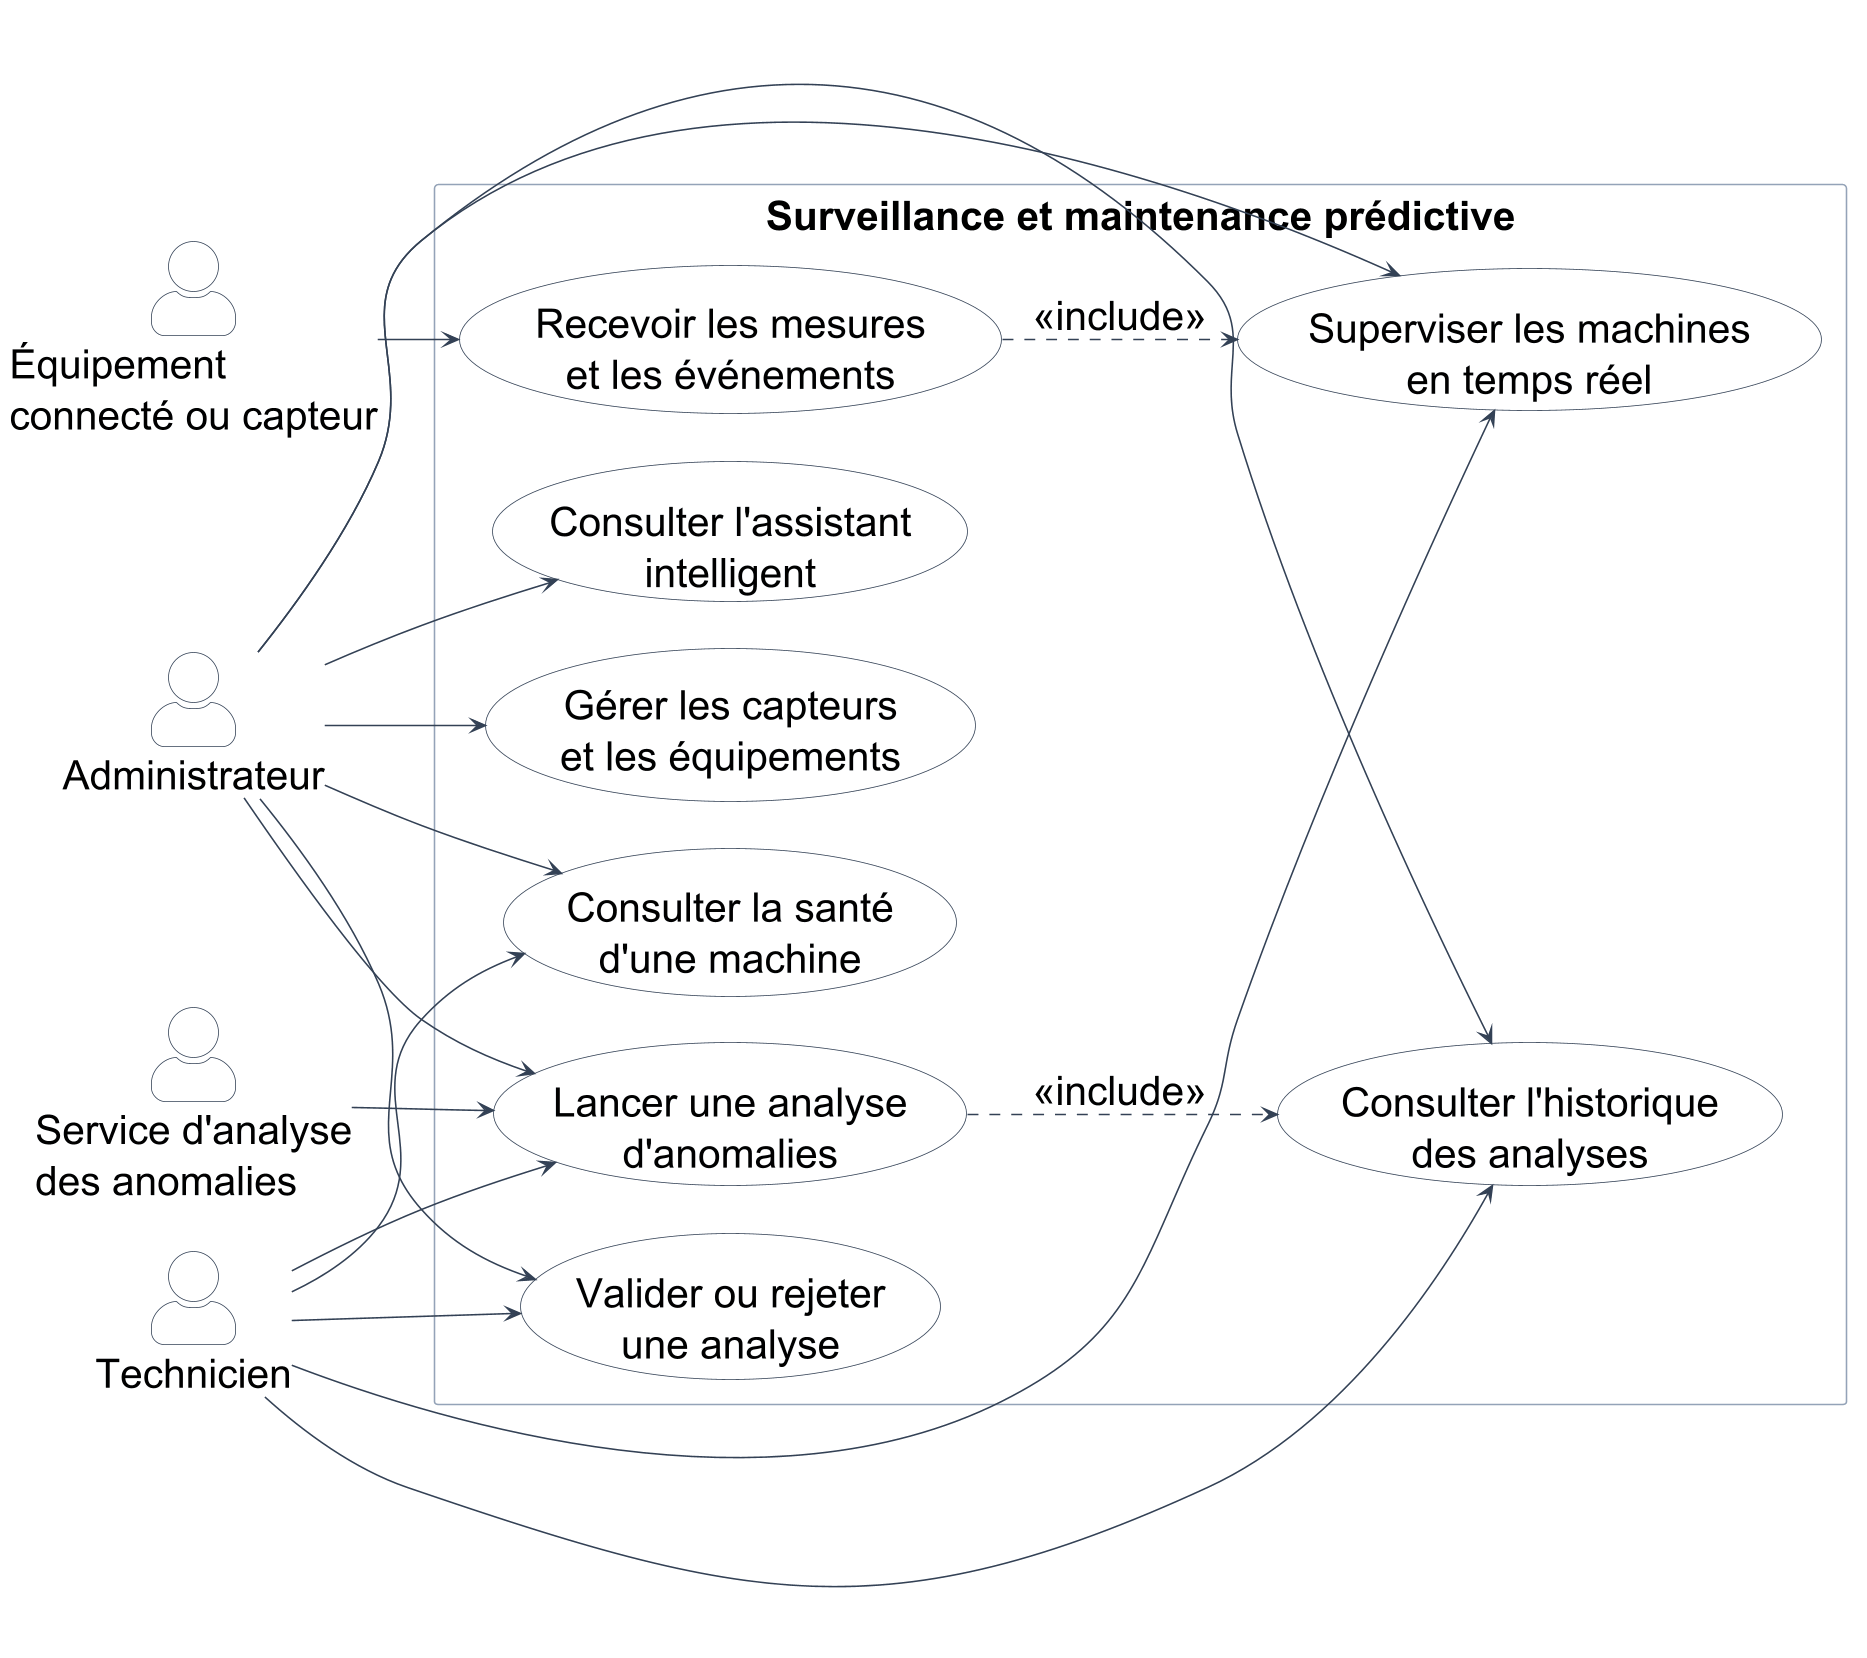
\includegraphics[width=0.70\textwidth,height=0.37\textheight,keepaspectratio]{figures/usecase-monitoring.png}%
    }{%
        \fbox{\parbox[c][7cm][c]{0.92\textwidth}{\centering\itshape Diagramme à insérer\\[2mm]\texttt{figures/usecase-monitoring.png}}}%
    }
    \caption{Diagramme des cas d'utilisation du Sprint 6}
    \label{fig:usecase-monitoring}
\end{figure}



\subsubsection{Architecture de la chaîne de surveillance}

\begin{figure}[H]
    \centering
    \IfFileExists{figures/architecture-monitoring.png}{%
        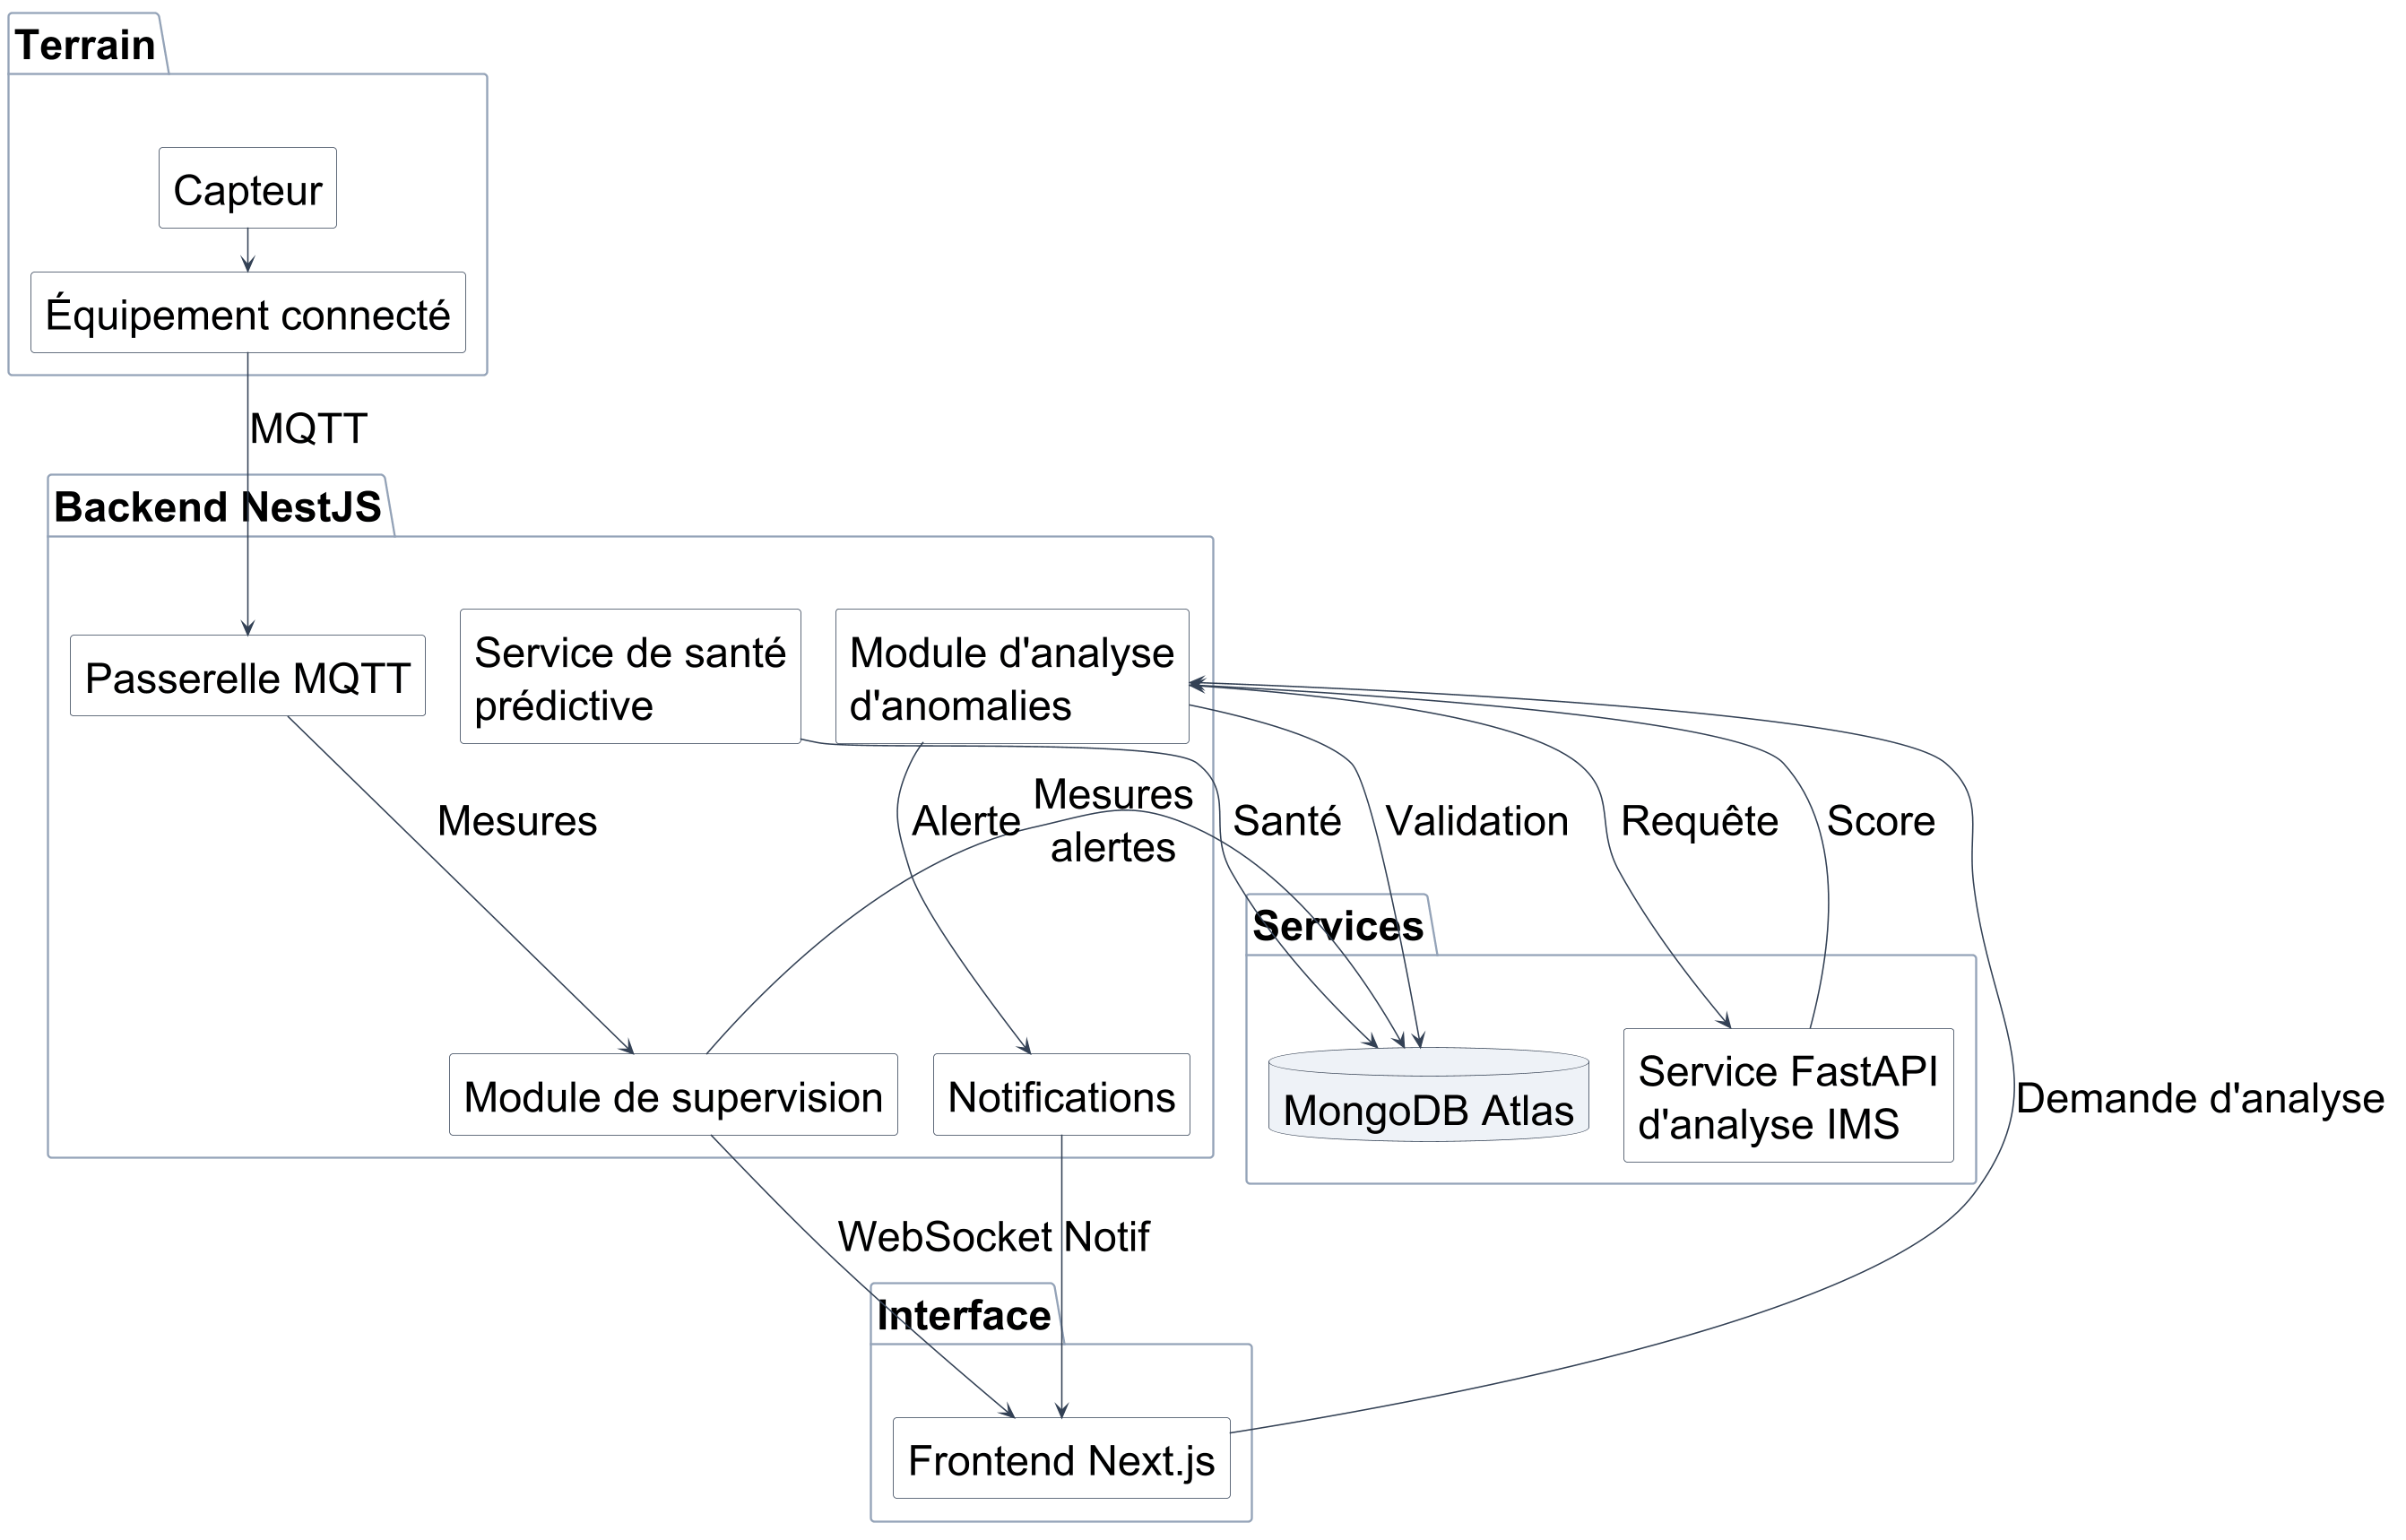
\includegraphics[width=0.92\textwidth,height=0.32\textheight,keepaspectratio]{figures/architecture-monitoring.png}%
    }{%
        \fbox{\parbox[c][7cm][c]{0.92\textwidth}{\centering\itshape Diagramme à insérer\\[2mm]\texttt{figures/architecture-monitoring.png}}}%
    }
    \caption{Architecture de la chaîne de surveillance et d'analyse}
    \label{fig:architecture-monitoring}
\end{figure}

La chaîne de surveillance relie les équipements du terrain, le backend NestJS, le service d'analyse FastAPI et les interfaces de supervision. La figure~\ref{fig:architecture-monitoring} présente cette organisation : les capteurs remontent leurs mesures à un équipement connecté qui publie des messages MQTT, la passerelle du backend acquiert ces messages puis les transmet au module de supervision. Ce dernier conserve les mesures et les alertes dans MongoDB, et diffuse les changements d'état au frontend Next.js par WebSocket. Le service de santé prédictive enregistre ses scores dans la même base. Lorsqu'une analyse est demandée depuis l'interface, le module d'anomalies du backend appelle le service FastAPI avec un jeton de service, conserve le résultat et la validation humaine, puis déclenche une notification si l'anomalie persiste.


\subsubsection{Diagramme de séquence de la collecte en temps réel}

La figure~\ref{fig:sequence-telemetry} présente la réception d'une mesure, son enregistrement et sa diffusion aux utilisateurs connectés. L'équipement publie le message sur le courtier MQTT, qui le transmet au backend. Celui-ci authentifie l'appareil et valide le contenu avant d'enregistrer la mesure et son statut dans MongoDB, puis de diffuser l'événement par la passerelle WebSocket afin de rafraîchir l'interface de supervision. Lorsque le message signale une panne, l'événement est conservé en tant qu'alerte et les utilisateurs abonnés reçoivent une notification.

\begin{figure}[H]
    \centering
    \IfFileExists{figures/sequence-telemetry.png}{%
        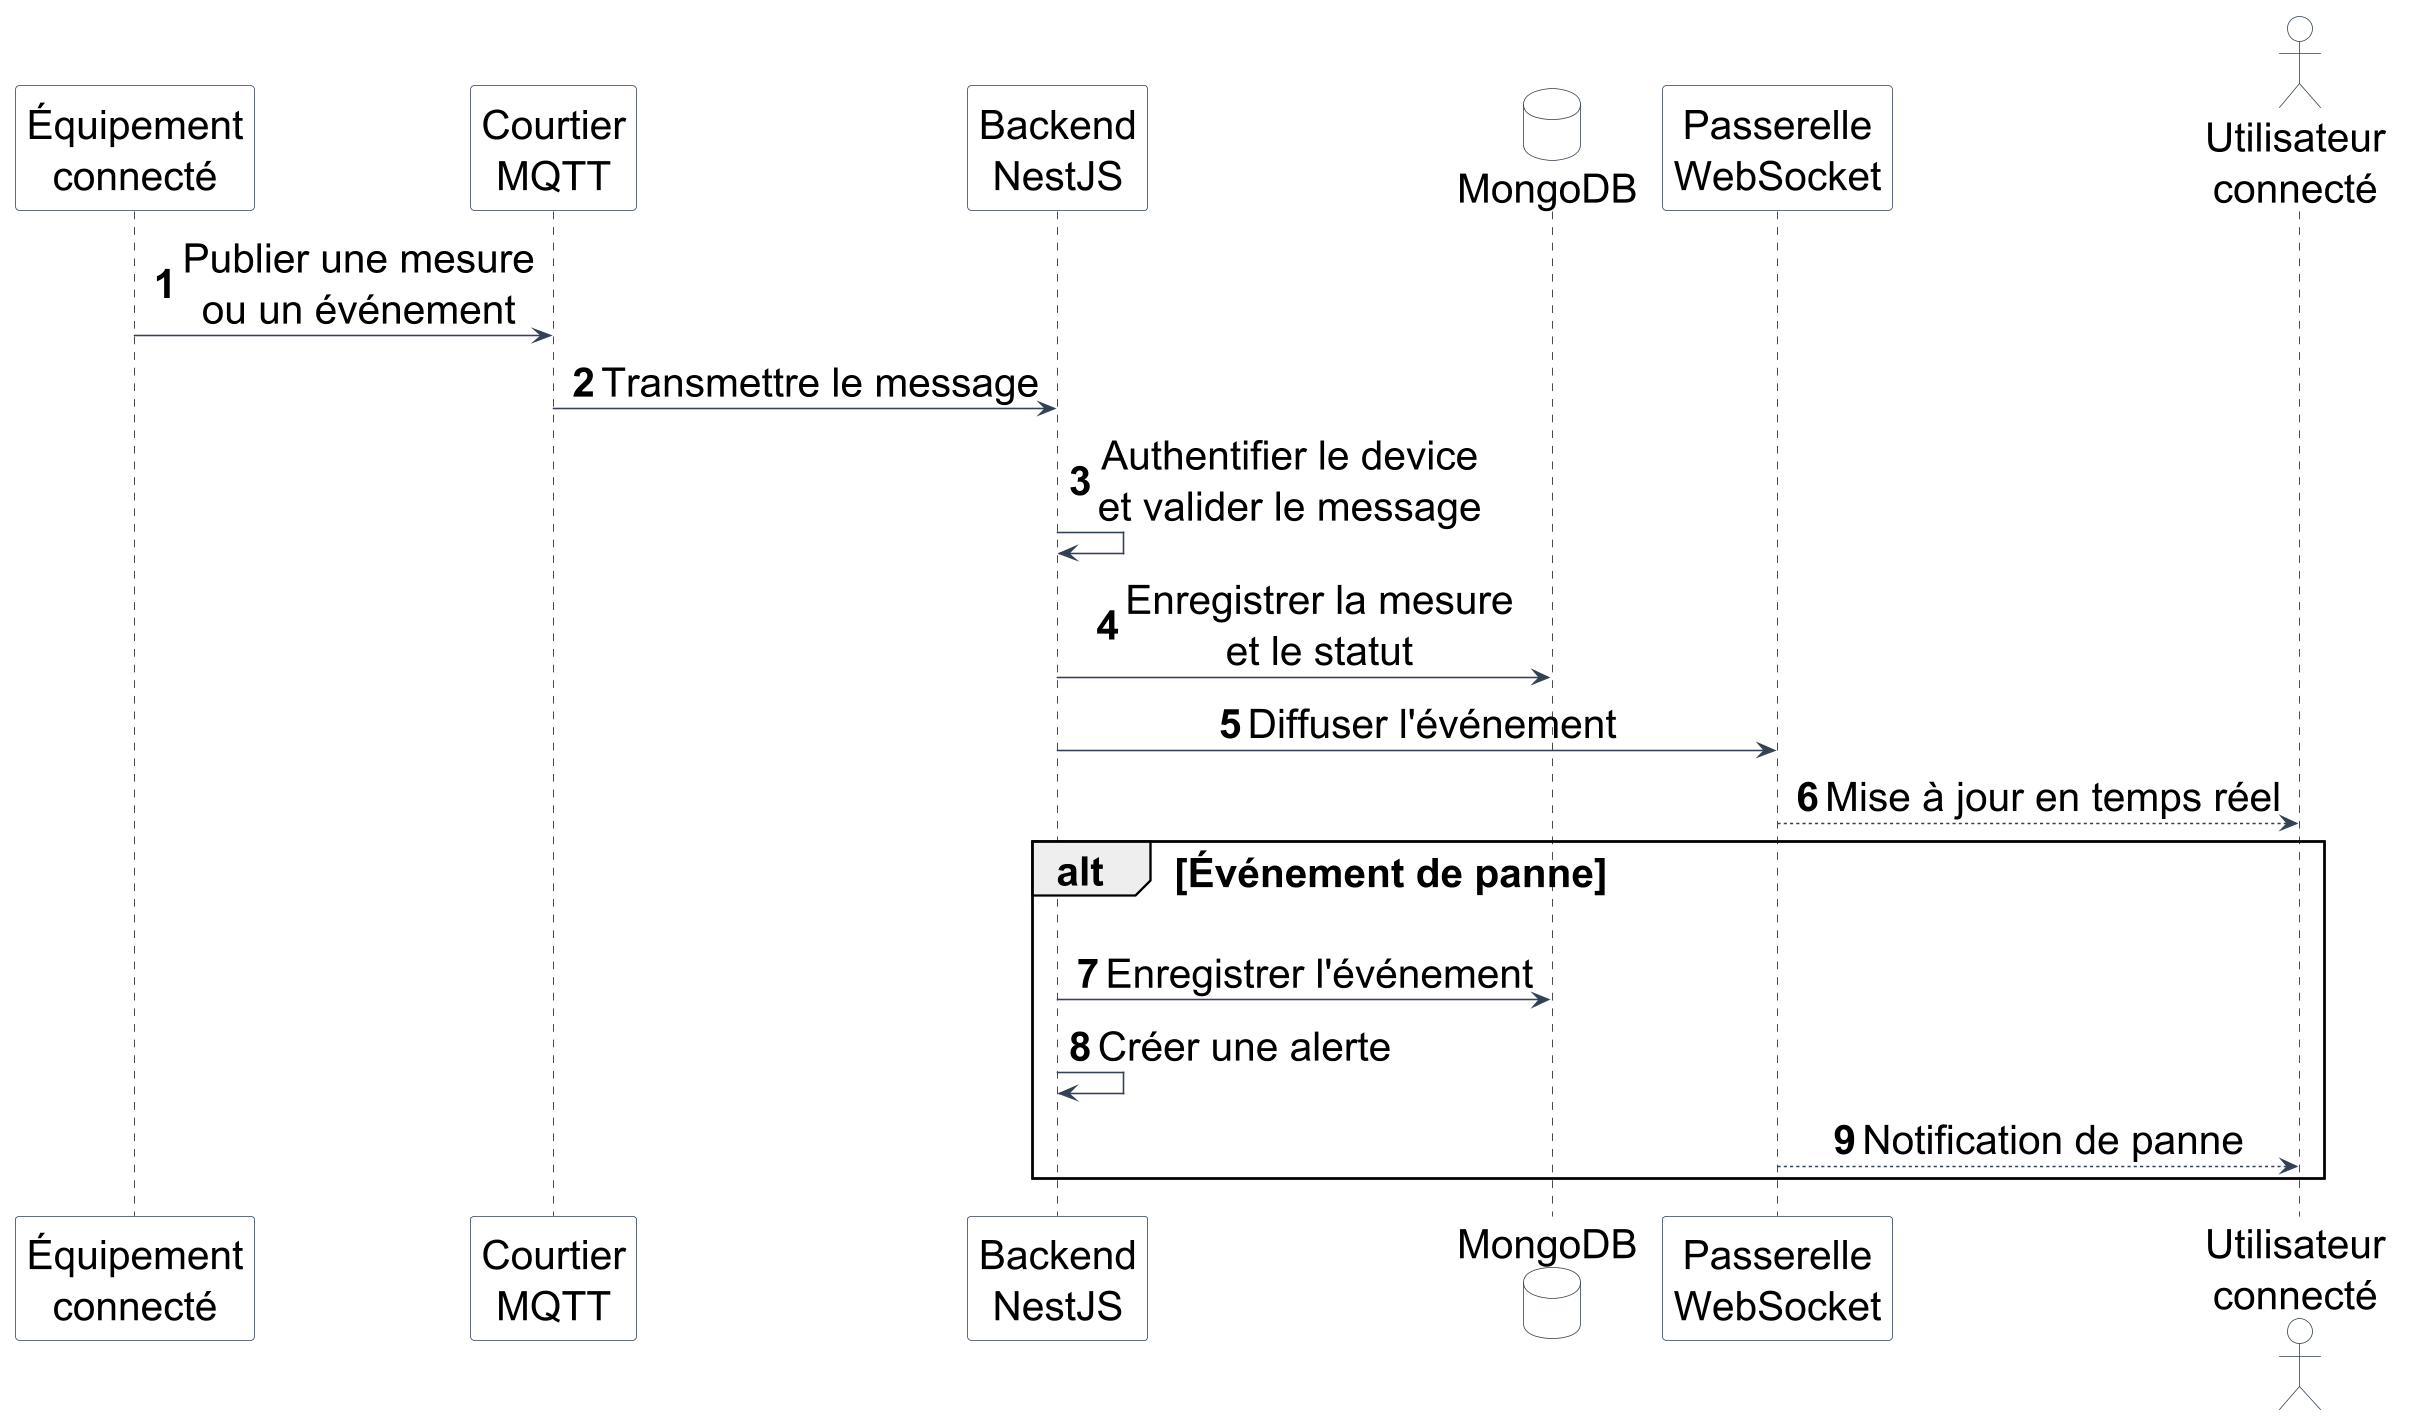
\includegraphics[width=\textwidth,height=0.40\textheight,keepaspectratio]{figures/sequence-telemetry.png}%
    }{%
        \fbox{\parbox[c][7cm][c]{0.92\textwidth}{\centering\itshape Diagramme à insérer\\[2mm]\texttt{figures/sequence-telemetry.png}}}%
    }
    \caption{Diagramme de séquence de la collecte et de la diffusion des mesures}
    \label{fig:sequence-telemetry}
\end{figure}


\subsubsection{Diagramme d'activités de l'ingestion des données}

La figure~\ref{fig:activity-telemetry} présente le traitement d'un message émis par un équipement. Le flux commence par le contrôle de l'identité de l'appareil, puis se poursuit par la validation du format, la conservation de la donnée et la diffusion de l'état aux utilisateurs abonnés. Une notification n'est créée que si un seuil est dépassé ou si une alarme reste active.
Les trois transports disponibles, à savoir l'API REST, le courtier MQTT et le canal WebSocket, convergent vers le même service d'ingestion. Cette convergence garantit que les règles de validation, de conservation et de notification restent identiques quel que soit le mode de transmission utilisé par l'équipement.

\begin{figure}[H]
    \centering
    \IfFileExists{figures/activity-telemetry.png}{%
        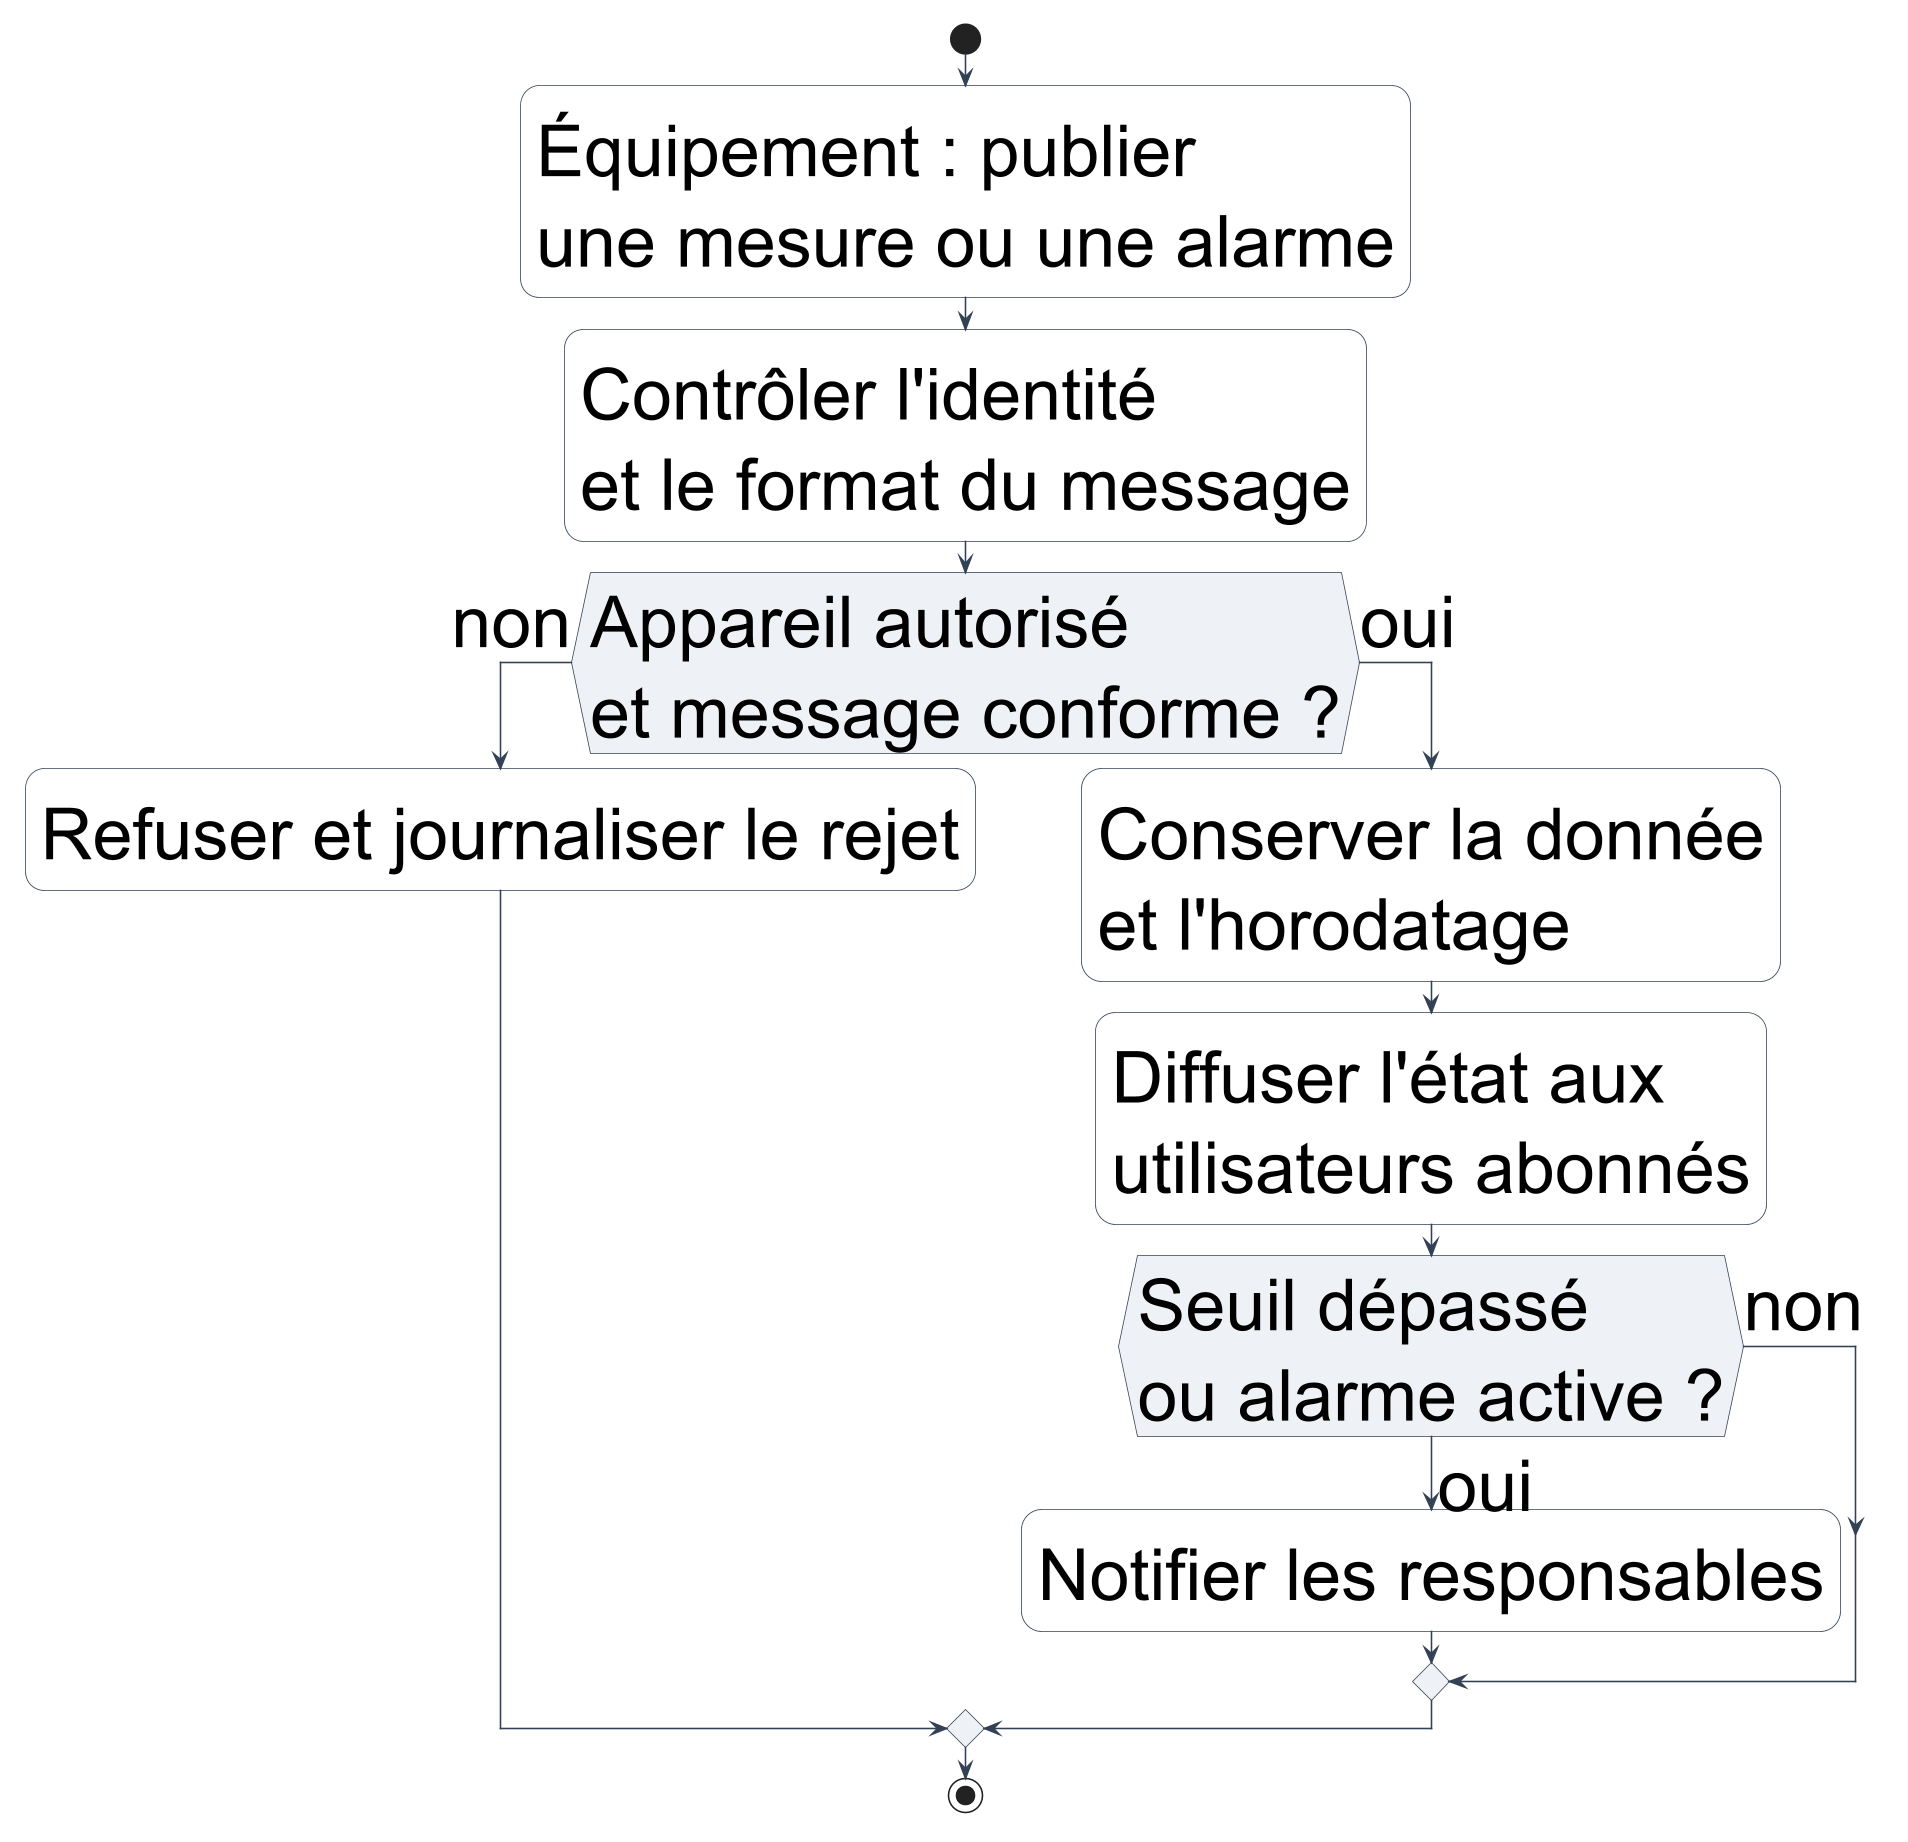
\includegraphics[width=0.60\textwidth,height=0.34\textheight,keepaspectratio]{figures/activity-telemetry.png}%
    }{%
        \fbox{\parbox[c][7cm][c]{0.92\textwidth}{\centering\itshape Diagramme à insérer\\[2mm]\texttt{figures/activity-telemetry.png}}}%
    }
    \caption{Diagramme d'activités de l'ingestion des données d'un équipement}
    \label{fig:activity-telemetry}
\end{figure}



\subsubsection{Diagramme de séquence de l'analyse d'anomalies}

\begin{figure}[H]
    \centering
    \IfFileExists{figures/sequence-anomaly.png}{%
        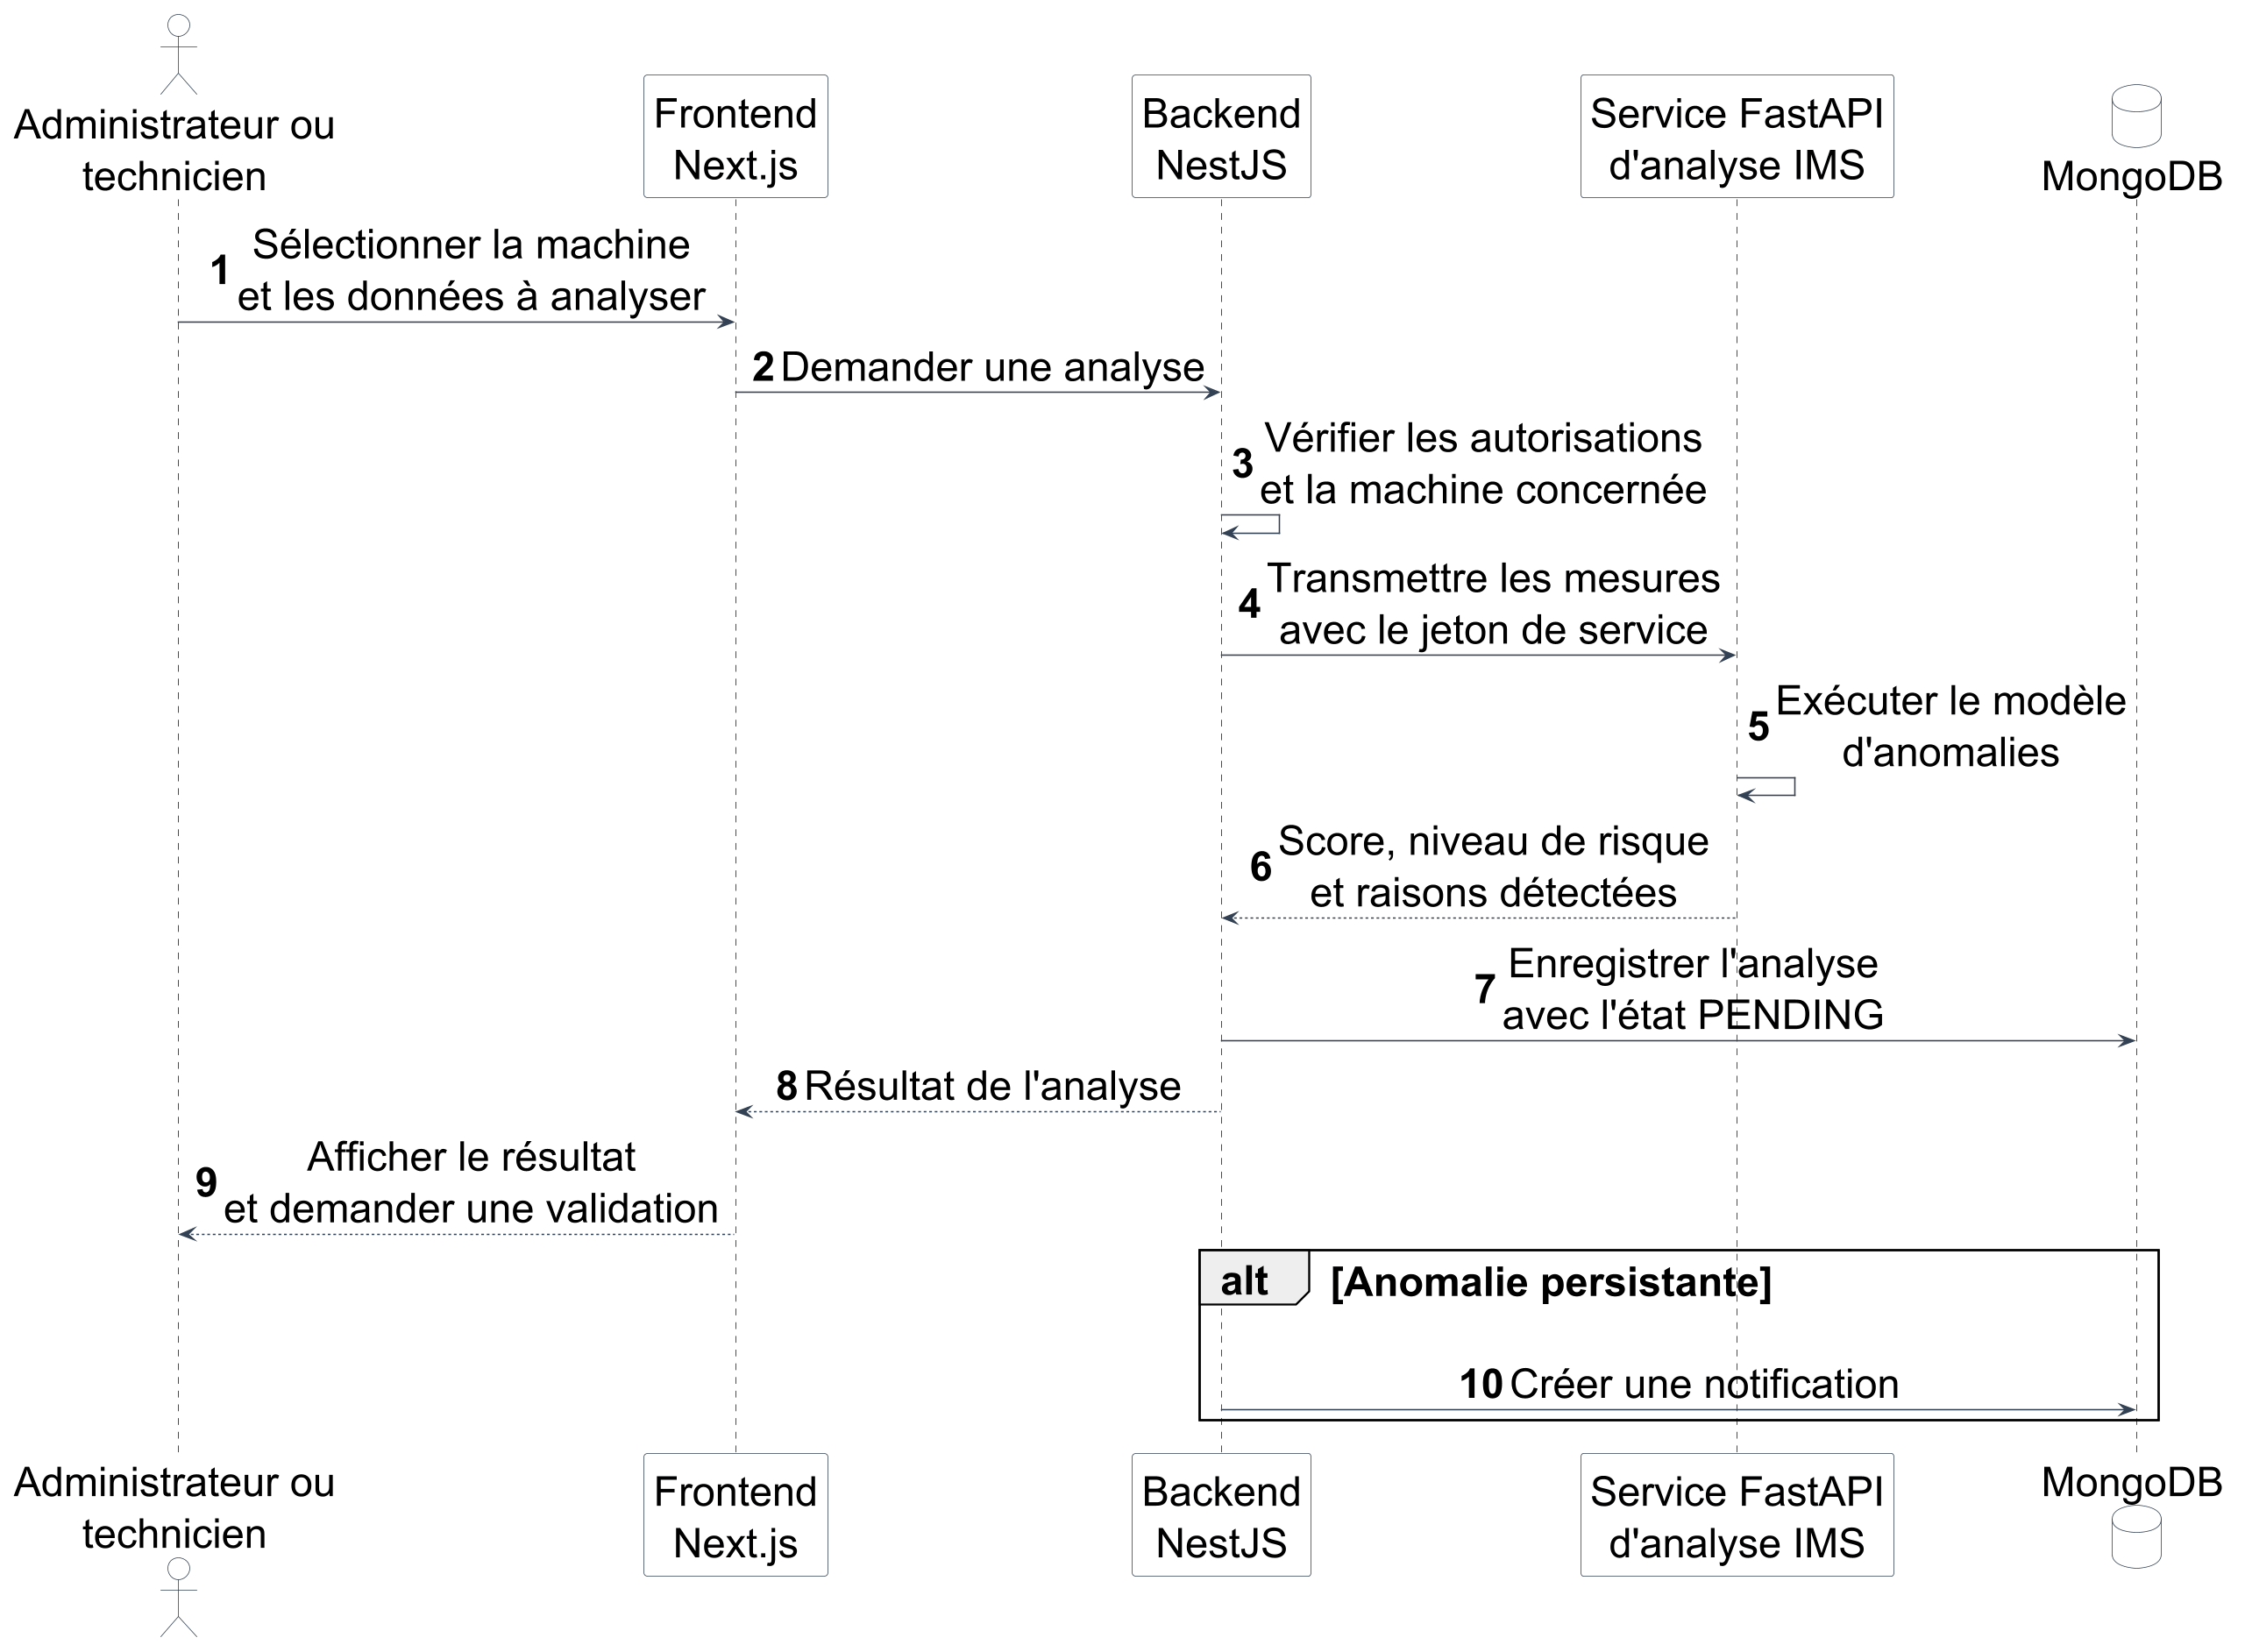
\includegraphics[width=0.70\textwidth,height=0.33\textheight,keepaspectratio]{figures/sequence-anomaly.png}%
    }{%
        \fbox{\parbox[c][7cm][c]{0.92\textwidth}{\centering\itshape Diagramme à insérer\\[2mm]\texttt{figures/sequence-anomaly.png}}}%
    }
    \caption{Diagramme de séquence de l'analyse d'anomalies}
    \label{fig:sequence-anomaly}
\end{figure}

L'analyse est déclenchée depuis l'interface. L'utilisateur sélectionne la machine et les données à analyser ; le backend vérifie ses autorisations et l'accès à la machine concernée, puis transmet les mesures au service FastAPI accompagnées du jeton de service. Le service exécute le modèle et renvoie un score, un niveau de risque et les raisons détectées. Le backend enregistre ensuite l'analyse avec l'état \texttt{PENDING} avant de restituer le résultat à l'interface, qui demande une validation. La figure~\ref{fig:sequence-anomaly} présente ce déroulement.
Lorsque la réponse signale une anomalie persistante, une notification est créée une seule fois. En cas d'indisponibilité du service ou de dépassement du délai d'attente, aucune analyse n'est enregistrée : l'utilisateur reçoit un message d'erreur explicite plutôt qu'un résultat partiel. Un rejeu du même échantillon met à jour l'analyse existante au lieu de créer un doublon.



\subsubsection{Diagramme d'états d'une analyse d'anomalie}

Chaque analyse est enregistrée avec un état de validation. À sa création, elle est à l'état \texttt{PENDING} : elle peut alors être confirmée si l'anomalie est avérée, ou rejetée s'il s'agit d'un faux positif ou d'une anomalie écartée. Ces deux états sont définitifs : le service refuse toute nouvelle validation, ce qui garantit que la décision consignée reste unique et attribuable à son auteur. La figure~\ref{fig:state-anomaly} présente ce cycle.

\begin{figure}[H]
    \centering
    \IfFileExists{figures/state-anomaly.png}{%
        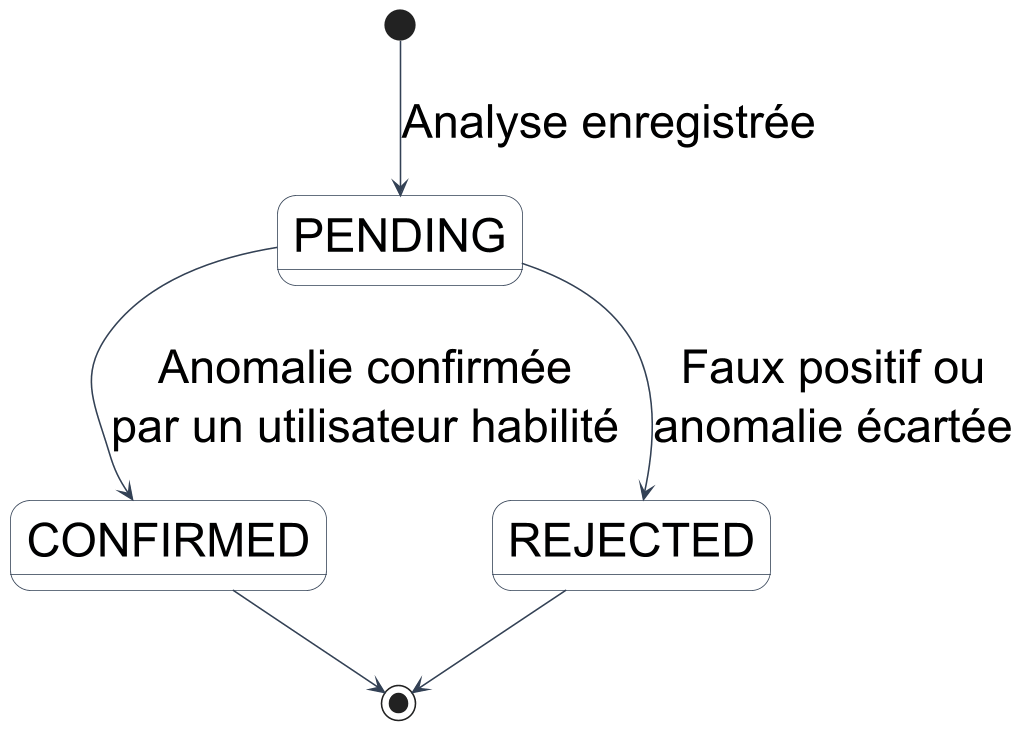
\includegraphics[width=0.66\textwidth,height=0.28\textheight,keepaspectratio]{figures/state-anomaly.png}%
    }{%
        \fbox{\parbox[c][7cm][c]{0.92\textwidth}{\centering\itshape Diagramme à insérer\\[2mm]\texttt{figures/state-anomaly.png}}}%
    }
    \caption{Diagramme d'états d'une analyse d'anomalie}
    \label{fig:state-anomaly}
\end{figure}



\subsubsection{Modèle de données de la surveillance}

Le tableau~\ref{tab:modele-monitoring} présente les principales entités du domaine de la surveillance.

\begin{table}[H]
\centering
\caption{Entités du domaine de la surveillance}
\label{tab:modele-monitoring}
\footnotesize
\setlength{\tabcolsep}{4pt}
\begin{tabularx}{\textwidth}{|>{\raggedright\arraybackslash}p{4.1cm}|>{\raggedright\arraybackslash}X|}
\hline
\textbf{Entité} & \textbf{Rôle dans le domaine} \\
\hline
\texttt{Device} & Équipement connecté transmettant des mesures et des événements, identifié par une clé propre et non réutilisable \\
\hline
\texttt{Capteur} & Dispositif de mesure rattaché à un module, avec son type, son unité, son sujet MQTT et ses seuils \\
\hline
\texttt{Mesure} & Valeur horodatée transmise par un capteur, avec son statut de réception \\
\hline
\texttt{Telemetry} & Lot de mesures transmis par un appareil, avec les dates d'enregistrement et de réception \\
\hline
\texttt{FaultEvent} & Alarme signalée par un appareil, éventuellement résolue par un utilisateur \\
\hline
\texttt{MachineHealthPrediction} & Indicateur de santé et niveau de risque d'une machine, accompagné de sa confiance \\
\hline
\texttt{AiAnomalyAnalysis} & Résultat d'une analyse, avec score, version du modèle, raisons détectées et état de validation \\
\hline
\texttt{Notification} & Alerte générée à la suite d'un événement ou d'une anomalie persistante \\
\hline
\texttt{AiInteraction} & Historique des échanges avec l'assistant intelligent, conservé pour l'audit \\
\hline
\end{tabularx}
\end{table}

Une analyse d'anomalie est associée à une machine et, lorsqu'il est identifié, à un capteur. Elle conserve la version du modèle utilisé, le score de risque, le niveau de risque, l'indicateur d'alerte persistante ainsi que l'auteur et la date de validation. Un index unique portant sur la machine, la version du modèle, la source, l'expérience, l'horodatage et le roulement empêche d'enregistrer deux fois le même résultat.
Deux mécanismes de prédiction coexistent dans la plateforme. Le premier s'appuie sur les modèles internes du backend, qui exploitent treize variables issues des mesures, des alarmes, des ordres de travail et des plans de maintenance. Le second s'appuie sur le service FastAPI, qui analyse des indicateurs vibratoires de roulements. Ces deux mécanismes produisent des résultats de nature différente et ne doivent pas être confondus : le premier estime l'état général d'une machine à partir de son activité de maintenance, le second détecte une signature d'anomalie dans un signal de roulement.

\subsection{Réalisation}

\subsubsection{Gestion des capteurs et des équipements connectés}

L'administrateur peut enregistrer un capteur, préciser son type et l'associer à un module. Il peut également gérer les équipements connectés et renouveler leur clé d'authentification.

Chaque capteur est décrit par un code, un type, une unité de mesure et, lorsque l'équipement le permet, un sujet MQTT. Il comporte des seuils d'avertissement et de critique, une fréquence d'échantillonnage et un indicateur d'activation ; la date de dernière activité distingue un capteur actif d'un capteur simplement déclaré.

Les équipements transmettent leurs données avec une authentification distincte de celle des utilisateurs. Cette séparation évite qu'un équipement puisse accéder aux fonctionnalités réservées aux comptes de maintenance. La clé de l'appareil n'est conservée que sous forme d'empreinte : elle n'est affichée en clair qu'une seule fois, lors de l'enregistrement ou de la rotation. Un appareil compromis ne peut donc pas accéder aux routes réservées aux utilisateurs, et un jeton d'utilisateur volé ne permet pas de publier des mesures.

Les capteurs peuvent être activés ou désactivés selon leur état de fonctionnement. Un capteur désactivé n'est plus pris en compte dans la collecte supervisée. L'administrateur peut également modifier l'intervalle de battement d'un appareil et consulter sa dernière activité.

\begin{figure}[H]
    \centering
    \IfFileExists{figures/sprint6-devices.png}{%
        \includegraphics[width=0.95\textwidth,height=0.82\textheight,keepaspectratio]{figures/sprint6-devices.png}%
    }{%
        \fbox{\parbox[c][7cm][c]{0.92\textwidth}{\centering\itshape Capture d'écran à insérer\\[2mm]\texttt{figures/sprint6-devices.png}}}%
    }
    \caption{Gestion des équipements connectés et de leur état}
    \label{fig:sprint6-devices}
\end{figure}

\subsubsection{Collecte et diffusion en temps réel}

Les mesures sont transmises par MQTT puis traitées par le backend. Chaque message est authentifié, validé et horodaté avant son enregistrement.

Les messages sont publiés sur des sujets préfixés par \texttt{devices/\{id\}/}, puis suffixés par \texttt{telemetry}, \texttt{heartbeat} ou \texttt{fault}. Le courtier MQTT repose sur un protocole de publication et d'abonnement adapté aux échanges de faible volume entre équipements \cite{mqtt_docs}. Il reste optionnel : en l'absence de configuration, le service ne se connecte pas et le reste de la plateforme continue de fonctionner. Les routes REST dédiées au battement, aux mesures et aux alarmes offrent le même traitement, protégées par une garde d'authentification propre aux appareils.

Chaque message est contrôlé avant conservation : identité de l'appareil, format des mesures, horodatage et bornes acceptables. Un appareil est considéré hors ligne lorsqu'il a manqué trois intervalles de battement consécutifs ; la notification correspondante n'est créée qu'à la transition d'état, et non à chaque balayage.

Les changements d'état sont diffusés par WebSocket aux utilisateurs connectés \cite{socketio_docs}. Cette diffusion permet d'actualiser les indicateurs sans rechargement manuel de la page. L'interface combine un instantané obtenu par appel REST et un flux temps réel : l'instantané fournit l'état initial, le flux pousse ensuite les mesures et les alarmes.

La supervision en direct présente l'état des machines, les dernières mesures reçues et les alertes actives. La résolution d'une alarme n'est pas automatique : elle reste une décision d'un utilisateur habilité, même lorsque l'équipement revient à un état normal.

La qualité de la surveillance dépend directement de celle des mesures reçues. Un capteur mal calibré, une alimentation instable ou une horloge déréglée produisent des valeurs aberrantes qui ressemblent à une anomalie sans qu'aucune défaillance ne soit réelle. Le contrôle du format et des bornes écarte les messages manifestement invalides sans remplacer une vérification périodique de l'instrumentation ; la conservation de l'horodatage d'enregistrement et de celui de réception permet de détecter un décalage d'horloge ou un envoi différé.

\begin{figure}[H]
    \centering
    \IfFileExists{figures/sprint6-live-monitoring.png}{%
        \includegraphics[width=0.95\textwidth,height=0.82\textheight,keepaspectratio]{figures/sprint6-live-monitoring.png}%
    }{%
        \fbox{\parbox[c][7cm][c]{0.92\textwidth}{\centering\itshape Capture d'écran à insérer\\[2mm]\texttt{figures/sprint6-live-monitoring.png}}}%
    }
    \caption{Supervision en temps réel de l'état des machines}
    \label{fig:sprint6-live-monitoring}
\end{figure}

\subsubsection{Indicateur de santé des machines}

La plateforme calcule un indicateur de santé pour chaque machine à partir des données disponibles. Cet indicateur synthétise l'état observé et permet de comparer les équipements d'une même flotte.

Il s'appuie sur treize variables décrivant l'activité récente : mesures, alarmes, ordres de travail et plans de maintenance. Le calcul produit un score, un niveau de risque et une date de génération ; l'historique des prédictions est conservé afin de suivre l'évolution de l'état d'une machine.

Le score est obtenu par la relation suivante :

\begin{equation}
H = 100 \times (1 - a)
\label{eq:health-score}
\end{equation}

où $a$ désigne le score d'anomalie produit par le modèle, compris entre 0 et 1. Un indicateur proche de 100 correspond à une machine dont l'activité ne présente pas d'écart notable.

Plusieurs modèles sont disponibles : un modèle fondé sur l'écart standardisé, une forêt d'isolement, un regroupement par densité et un autoencodeur. La version utilisée est conservée avec chaque prédiction, ainsi que le niveau de confiance et une explication des variables ayant contribué au résultat. Les prédictions sont recalculées par une tâche planifiée quotidienne et peuvent être rafraîchies à la demande pour une machine donnée.

L'indicateur est présenté comme une aide au suivi. Il ne constitue pas une mesure de sécurité ni une décision automatique d'arrêt de production. Lorsque les données sont insuffisantes, le niveau de risque prend la valeur \texttt{insufficient\_data} plutôt que de laisser croire à un état sain.

\subsubsection{Service d'analyse des anomalies}

Le service d'analyse est développé avec FastAPI et exécuté indépendamment du backend. Il charge un modèle d'apprentissage automatique destiné à détecter des comportements anormaux sur des données de roulements.

Le backend transmet les mesures au service avec un jeton de service. Le service renvoie un score, un niveau de risque et les raisons associées à la détection. Ces informations sont enregistrées puis présentées à l'utilisateur.

Le service prend en charge deux modes d'analyse :

\begin{itemize}
    \item une analyse ponctuelle à partir d'un ensemble de mesures ;
    \item une analyse par lot sur plusieurs observations.
\end{itemize}

Le modèle est chargé depuis un artefact versionné, ce qui permet de connaître la version utilisée pour chaque analyse. Le service ne réentraîne jamais un modèle pendant une requête : il charge un artefact figé, identifié par sa version. L'accès est protégé par un jeton de service transmis dans un en-tête dédié et comparé en temps constant, afin d'éviter une attaque par mesure du temps de réponse.

Une anomalie n'est signalée comme persistante que si elle se répète sur une fenêtre glissante. Cette exigence limite les alertes isolées. Le tableau~\ref{tab:metriques-anomalie} présente les principaux indicateurs du protocole d'évaluation.

{\footnotesize
\setlength{\tabcolsep}{4pt}
\begin{table}[H]
\centering
\caption{Indicateurs d'évaluation du modèle d'anomalies (version 0.2.0)}
\label{tab:metriques-anomalie}
\begin{tabularx}{\textwidth}{|>{\raggedright\arraybackslash}p{5.6cm}|>{\raggedright\arraybackslash}p{1.6cm}|>{\raggedright\arraybackslash}X|}
\hline
\textbf{Indicateur} & \textbf{Valeur} & \textbf{Lecture} \\
\hline
Précision & 0,487 & Part des alertes correspondant à une défaillance proche \\
\hline
Rappel & 0,281 & Part des défaillances détectées avant l'arrêt \\
\hline
F1 & 0,356 & Compromis entre précision et rappel \\
\hline
Aire sous la courbe ROC & 0,709 & Capacité de discrimination globale \\
\hline
Faux positifs par jour & 0,907 & Charge de vérification induite pour les techniciens \\
\hline
Délai médian de détection & 390 h & Anticipation médiane avant la défaillance \\
\hline
\end{tabularx}
\end{table}}

Ces résultats appellent une réserve importante : le modèle ne mesure pas une durée de vie résiduelle et ne se substitue pas à une expertise de surveillance conditionnelle \cite{iso13374}. Ses limites sont détaillées dans la sous-section~\ref{subsec:limites-modele}.

\subsubsection{Validation humaine des résultats}

Les analyses sont initialement enregistrées avec l'état \texttt{PENDING}. Un administrateur ou un technicien disposant des droits nécessaires peut les consulter puis les confirmer ou les rejeter.

La confirmation indique que l'anomalie est jugée pertinente au regard du contexte de la machine. Le rejet permet d'écarter un faux positif ou une situation déjà expliquée.

Chaque décision conserve son auteur et sa date. Ce mécanisme garantit que les résultats du modèle ne sont pas utilisés comme des décisions automatiques et qu'une expertise humaine reste associée à toute action de maintenance. Le système refuse une seconde validation : une analyse déjà traitée ne peut plus changer d'état, ce qui évite qu'un même résultat soit successivement confirmé et rejeté par deux utilisateurs.

\begin{figure}[H]
    \centering
    \IfFileExists{figures/sprint6-anomaly-analysis.png}{%
        \includegraphics[width=0.95\textwidth,height=0.82\textheight,keepaspectratio]{figures/sprint6-anomaly-analysis.png}%
    }{%
        \fbox{\parbox[c][7cm][c]{0.92\textwidth}{\centering\itshape Capture d'écran à insérer\\[2mm]\texttt{figures/sprint6-anomaly-analysis.png}}}%
    }
    \caption{Analyse d'anomalies et validation par un utilisateur habilité}
    \label{fig:sprint6-anomaly-analysis}
\end{figure}

\subsubsection{Notifications et alertes persistantes}

Lorsqu'une anomalie est détectée de manière persistante, une notification est créée à destination des utilisateurs concernés. La notification précise la machine, le niveau de risque et la date de l'analyse.

Une clé de déduplication empêche la création de plusieurs notifications pour la même analyse. Le message signale qu'il s'agit d'un rejeu de données expérimentales et non d'une mesure réelle, afin d'éviter toute confusion lors de la démonstration.

Les alertes persistantes sont distinguées des événements ponctuels afin d'éviter la multiplication de notifications pour un même phénomène. La notification est adressée aux administrateurs et aux techniciens et ouvre la fiche de la machine concernée ; l'analyse correspondante y est ensuite consultée dans l'historique.

La résolution d'une alarme signalée par un équipement suit un mécanisme distinct. Un utilisateur habilité déclenche la résolution depuis la supervision et peut y joindre une note, facultative mais limitée en longueur. L'alarme quitte alors la liste des alarmes actives tout en restant consultable dans l'historique, avec son auteur et sa date de résolution ; une seconde résolution est refusée.

\subsubsection{Assistant intelligent}

La plateforme propose un assistant fondé sur un service d'intelligence artificielle externe. Cette fonctionnalité est optionnelle et doit être activée par configuration. Elle s'appuie sur l'historique des interventions, le référentiel des pannes et les documents indexés dans la base de connaissances.

Lorsqu'elle est disponible, l'assistant peut aider l'utilisateur à consulter les informations de maintenance, à interpréter un contexte ou à retrouver une procédure. Les échanges sont conservés dans un historique associé à l'utilisateur, à la machine et éventuellement à l'ordre de travail.

L'assistant ne dispose pas d'un accès direct aux données sans passer par le backend. Les secrets du fournisseur restent conservés côté serveur et ne sont jamais exposés au navigateur. Lorsque la fonctionnalité est désactivée, un fournisseur neutre répond que l'assistance n'est pas disponible, sans bloquer le reste du flux correctif ; lorsqu'elle est activée avec le fournisseur Gemini \cite{gemini_api}, une configuration incomplète est signalée explicitement plutôt que d'échouer silencieusement.

Plusieurs garde-fous encadrent son usage. Un quota horaire limite le nombre de sollicitations par utilisateur. Un filtre retire les données sensibles du contexte transmis. Un mécanisme de protection contre l'injection de consignes traite le contenu des documents comme une donnée et non comme une instruction. Enfin, les sources documentaires utilisées sont renvoyées avec la réponse, ce qui permet à l'utilisateur de vérifier l'origine d'une recommandation.

\subsubsection{Limites actuelles du modèle}
\label{subsec:limites-modele}

Le modèle d'anomalies intégré est un prototype validé sur un jeu de données public relatif à des roulements, IMS Bearing \cite{nasa_ims}, issu d'un banc d'essai. Sa généralisation aux équipements de production d'IPROTEX n'a pas encore été établie. Les étiquettes de défaillance de ce jeu sont des proxys temporels et non des annotations fiables à l'échelle de l'horodatage.

Les résultats produits doivent donc être interprétés comme des indications à examiner et non comme des seuils de sécurité industrielle certifiés. Le seuil d'admission en pilote consultatif n'est pas atteint pour cette version. Une phase complémentaire serait nécessaire pour collecter des données représentatives des machines de l'entreprise, réentraîner le modèle et mesurer ses performances dans les conditions réelles d'exploitation.

Cette limite est explicitement présentée dans l'interface et dans le rapport afin d'éviter toute confiance excessive dans les prédictions. Elle justifie le maintien d'une validation humaine systématique et interdit tout déclenchement automatique d'une intervention à partir du seul score.


\subsection{Tests et validation}

Le tableau~\ref{tab:tests-sprint6} présente les scénarios de test retenus pour ce Sprint.

{\footnotesize
\setlength{\tabcolsep}{4pt}
\begin{longtable}{|p{0.9cm}|>{\raggedright\arraybackslash}p{7cm}|>{\raggedright\arraybackslash}p{4.7cm}|}
\caption{Scénarios de test du Sprint 6}
\label{tab:tests-sprint6}\\
\hline
\textbf{ID} & \textbf{Scénario} & \textbf{Résultat attendu} \\
\hline
\endfirsthead

\hline
\textbf{ID} & \textbf{Scénario} & \textbf{Résultat attendu} \\
\hline
\endhead

T6-01 &
Création d'un capteur rattaché à un module &
Capteur enregistré et visible dans la liste \\
\hline

T6-02 &
Enregistrement d'un équipement connecté &
Clé affichée une seule fois et empreinte seule conservée \\
\hline

T6-03 &
Rotation de la clé d'un équipement &
Ancienne clé refusée, nouvelle clé acceptée \\
\hline

T6-04 &
Transmission d'une mesure avec une clé invalide &
Message rejeté et non conservé \\
\hline

T6-05 &
Transmission d'une mesure par MQTT &
Mesure conservée et dernière activité mise à jour \\
\hline

T6-06 &
Transmission d'une mesure par l'API REST &
Même traitement que par MQTT \\
\hline

T6-07 &
Diffusion d'un changement d'état par WebSocket &
Utilisateur abonné notifié pour la machine concernée \\
\hline

T6-08 &
Absence de battement au-delà de trois intervalles &
Équipement marqué hors ligne et notification unique \\
\hline

T6-09 &
Signalement d'une alarme par un équipement &
Alarme active et compteur d'alarmes mis à jour \\
\hline

T6-10 &
Résolution d'une alarme par un technicien &
Alarme retirée des alarmes actives et note conservée \\
\hline

T6-11 &
Lancement d'une analyse avec un accès autorisé &
Analyse enregistrée au statut en attente \\
\hline

T6-12 &
Appel du service sans jeton de service &
Réponse d'authentification refusée \\
\hline

T6-13 &
Indisponibilité du service d'analyse &
Erreur explicite et aucune analyse partielle enregistrée \\
\hline

T6-14 &
Confirmation d'une analyse déjà validée &
Seconde validation refusée \\
\hline

T6-15 &
Détection d'une anomalie persistante &
Notification créée une seule fois pour l'analyse \\
\hline

T6-16 &
Consultation d'une machine sans donnée exploitable &
Niveau de risque \texttt{insufficient\_data} affiché \\
\hline

T6-17 &
Consultation de l'assistant lorsqu'il est désactivé &
Message explicite sans blocage du flux correctif \\
\hline

\end{longtable}}

Les tests confirment la cohérence de la chaîne : une mesure transmise par MQTT ou par l'API REST produit le même enregistrement. Aucune analyse n'est conservée si le service échoue, la validation n'est acceptée qu'une fois et la déduplication empêche les notifications répétées.

\subsection{Revue du Sprint et conclusion}

Lors de la revue, l'enregistrement d'un équipement, la transmission de mesures, la supervision en temps réel, le lancement d'une analyse et sa validation ont été présentés.

Les principaux résultats sont les suivants :

\begin{itemize}[nosep,leftmargin=1.2em]
    \item capteurs et équipements connectés, avec des clés distinctes de celles des utilisateurs ;
    \item ingestion des mesures et des alarmes par REST, MQTT et WebSocket, en temps réel ;
    \item indicateur de santé, analyse des anomalies, validation humaine et notifications.
\end{itemize}

La rétrospective a souligné la différence de nature entre les deux mécanismes de prédiction : l'indicateur de santé résume l'activité de maintenance, le modèle d'anomalies analyse un signal vibratoire. Ce dernier reste un prototype de recherche évalué sur un jeu de données public, non prescriptif en l'état.

Le Sprint 7 sera consacré au déploiement et à la démarche DevSecOps.
